\documentclass[10pt,a4paper]{scrartcl}
\pagestyle{empty}
\usepackage{a4} % alternativ \usepackage{a4wide}
\usepackage[ngerman]{babel} % Neudeutsche Silbentrennung (mehrsprachiges Dokument)
\usepackage{parskip} % Skip indentation of first row
\usepackage{graphicx} % Graphics support
\usepackage{longtable} % Tables across several pages
\usepackage{booktabs}
\usepackage{hyperref} % Hyperlinks
\usepackage[automark]{scrpage2} %kopf/fusszeile
\usepackage[utf8x]{inputenc} % Unicode-Encoding
 
\linespread{1.3}

\author{Danilo Bargen, Christian Fässler, Jonas Furrer} 
\title{Code-Metriken und Design-Analyse Backend\\ Projekt BierIdee}

\pagestyle{scrheadings}
\ihead{SE2 Projekte} %linke Kopfzeile
\ohead{BierIdee} %rechte Kopfzeile

\begin{document}

\begin{titlepage}
	\maketitle
	\vspace{120mm}
	\thispagestyle{empty} % Don't start page numbers on this page
\end{titlepage}

\tableofcontents
\newpage

\section*{Änderungshistorie}
\begin{tabular}{p{0.1\textwidth}p{0.15\textwidth}p{0.55\textwidth}p{0.1\textwidth}}
\toprule
\textbf{Version} & \textbf{Datum} & \textbf{Änderung} & \textbf{Person} \\  
\midrule
v1.0 & 08.05.2012 & Dokument erstellt & jfurrer \\  
\midrule
v1.1 & 08.26.2012 & Dokument ergänzt & jfurrer \\  
\bottomrule
\end{tabular} 
\newpage

\section{Einführung}

\subsection{Zweck}
In diesem Dokument werden die Code Metriken des Projektes BierIdee zusammengetragen und betrachtet.

\subsection{Gültigkeitsbereich}
Die Gültigkeit des Dokumentes beschränkt sich auf die Dauer des SE2-Projekte Modules FS2012. Das
Dokument muss unter Berücksichtigung des Wachstums der Code-Basis ergänzt und erweitert werden.

\subsection{Tools}
Für die Analyse werden die folgende Tools verwendet:\\
\begin{itemize}
	\item Checkstyle
	\item Metrics Eclipse Plugin
	\item AnalytiX CodePro Tools
	\item Object Aid
\end{itemize}

\newpage

\section{Package Diagramm}
\subsection{Backend}
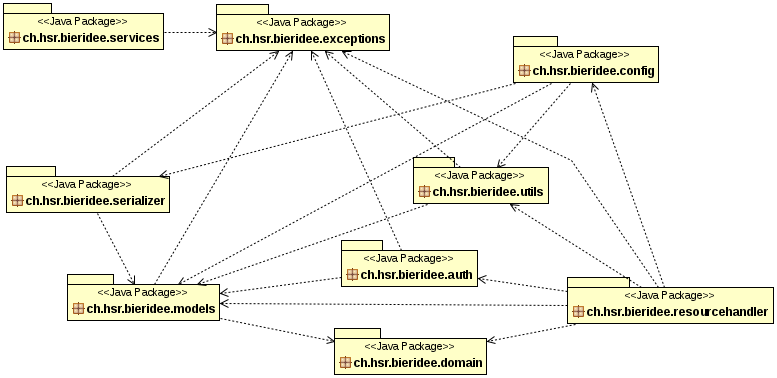
\includegraphics[width=\textwidth]{Package-Diagramm-Back.png}\\
\\
Die Packages zeigt die Stuktur des Backends deutlich auf, die Resource-Handler greifen  
auf die Models zu um Daten zu lesen und zu Persisteren. Dazwischen liegt noch das Auth package, dass für die Authentisierung nötig ist. Die Models greifen dann über Utilities
auf die Daten zu und persistieren die Domainobjekte.\\
Die Konfigurationen aus dem Config Package sowie die Exceptions werden von den meisten anderen
Packages benötigt.

\subsection{Frontend}
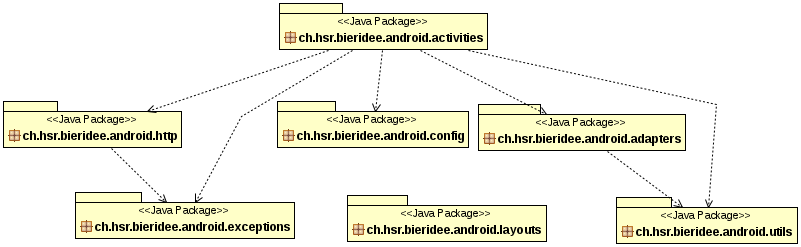
\includegraphics[width=\textwidth]{Package-Diagramm-Front.png}\\
\\
Die Struktur der Packages im Frontend zeigt den schichtartigen Aufbau wie er von den Android-Best-Practices vorgegeben wird.

\section{External Dependencies}
\subsection{Backend}
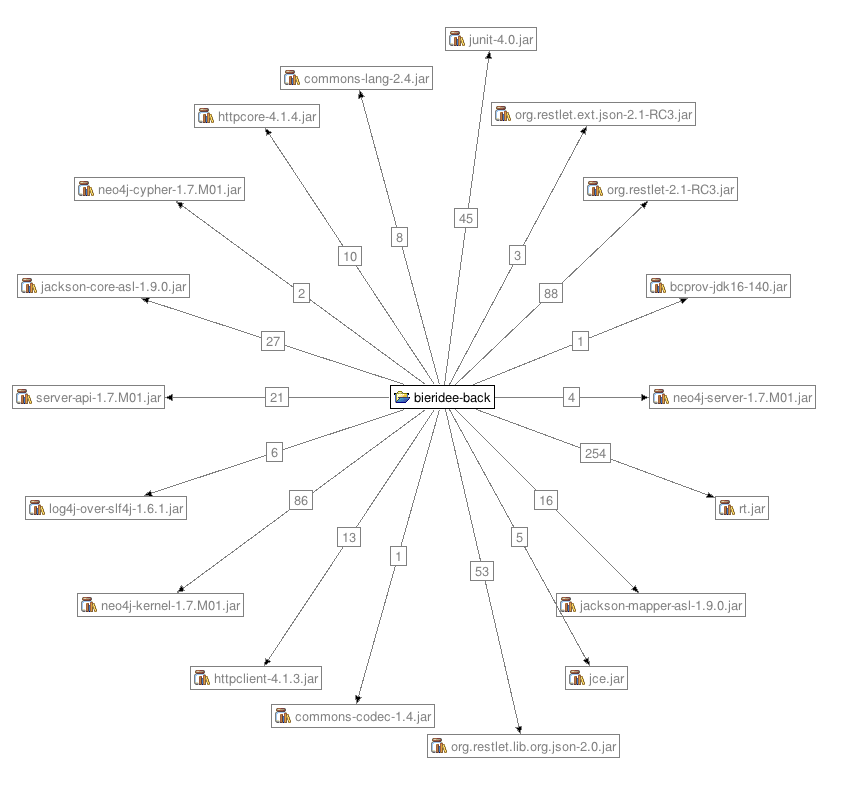
\includegraphics[scale=0.7, width=\textwidth]{External-Dependecies-Back.png}\\
\\
Durch die Verwendung von Restlet enstehen relativ viele externe Abhängigkeiten. 
\subsection{Frontend}
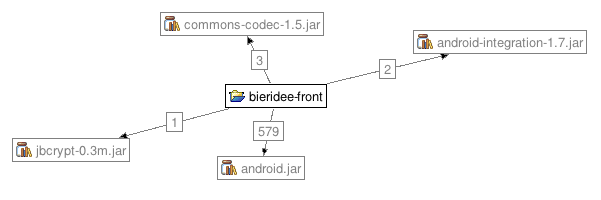
\includegraphics[width=\textwidth]{External-Dependecies-Front.png}\\
\\
Das Frontend ist sehr schlank, grundsätzlich auf Android Libraries zurückgegriffen werden kann.


\section{Metriken}
\subsection{Backend}
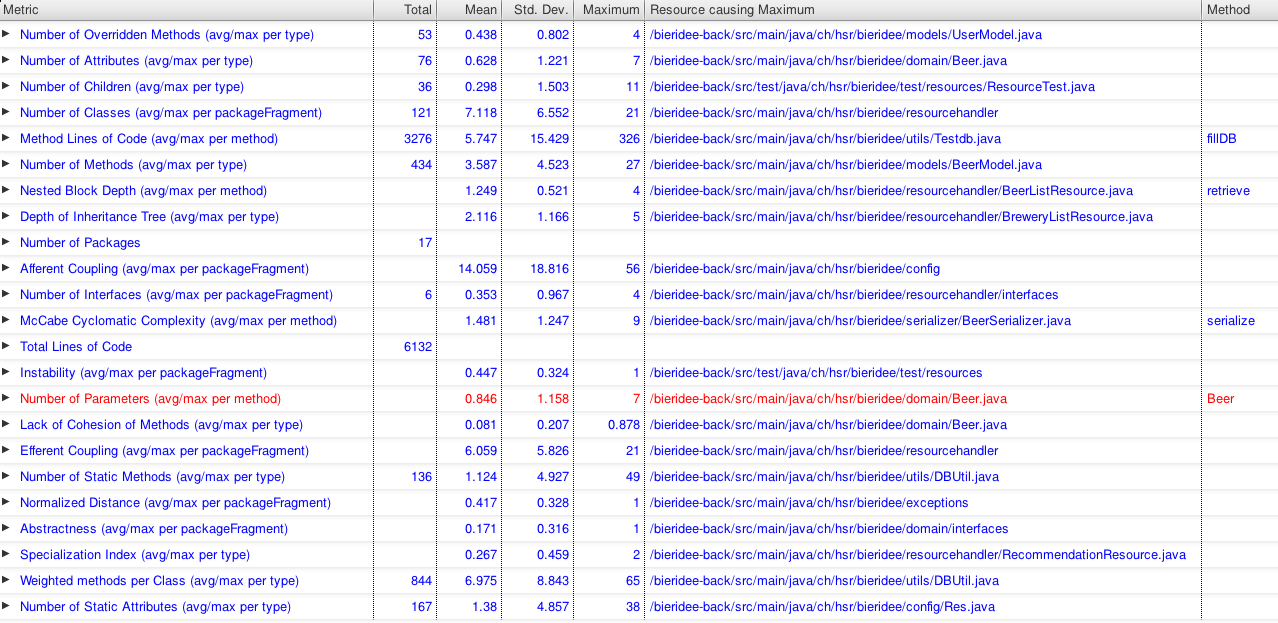
\includegraphics[scale=0.4, angle=90]{metrics-back.png}

Die einzige Metrik die im Backend einen kritischen Wert annimmt ist \"Numbers of Parameters\". Der Konstruktor des Beer Domain Objektes nimmt alls Parameter sämmtliche sieben Attribute an.
\newpage
\subsection{Frontend}
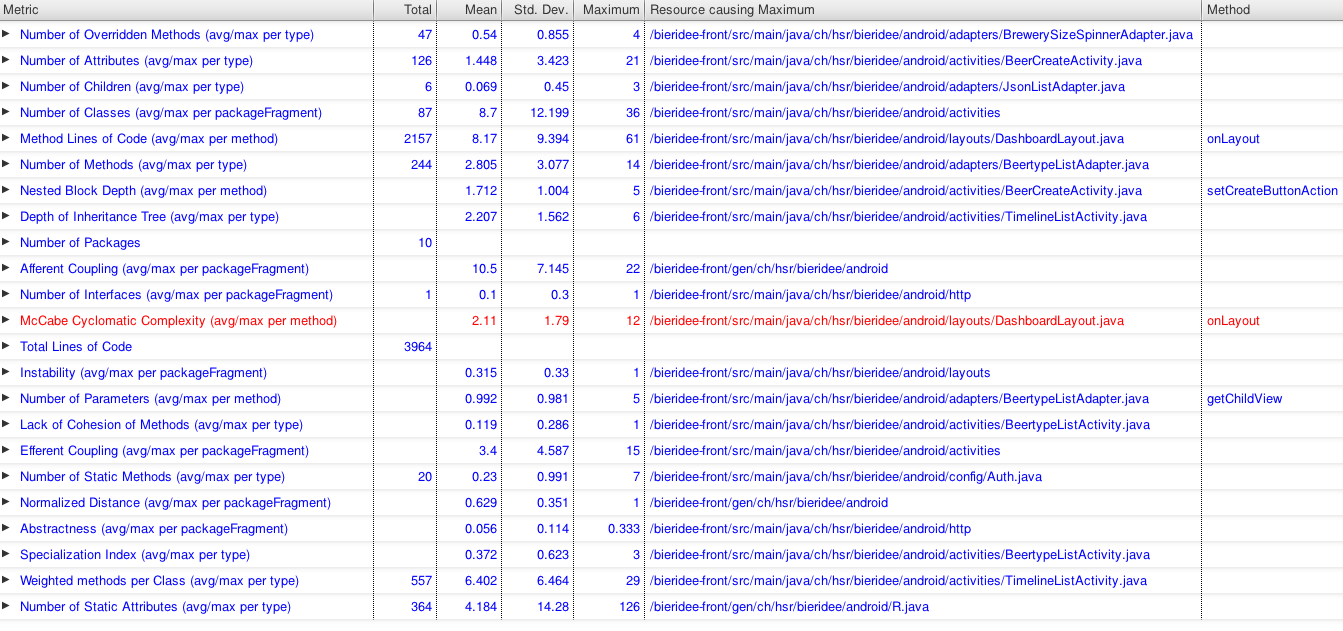
\includegraphics[scale=0.4, angle=90]{metrics-front.png}

Im Frontend ist ebenfalls nur eine Metrik als kritisch markiert. Bei der markierten Klasse handelt es sich um eine Klasse die von Google zur verfügung gestellt wird, deshalb ist diese Warnung für unsere Betrachtung nicht relevant.

\end{document}
